
%(BEGIN_QUESTION)
% Copyright 2006, Tony R. Kuphaldt, released under the Creative Commons Attribution License (v 1.0)
% This means you may do almost anything with this work of mine, so long as you give me proper credit

The venerable {\it orifice plate} is but one of many different pressure-generating primary sensing elements (PSE's) for flow measurement.  Briefly describe how each of these flow PSEs work, and how they compare against orifice plates in terms of application and performance:

$$\includegraphics[width=15.5cm]{i00479x01.eps}$$

\vskip 10pt

$$\includegraphics[width=15.5cm]{i00479x02.eps}$$

\vskip 10pt

$$\includegraphics[width=15.5cm]{i00479x03.eps}$$

\vskip 10pt

$$\includegraphics[width=15.5cm]{i00479x04.eps}$$

\vskip 10pt

$$\includegraphics[width=15.5cm]{i00479x05.eps}$$

\vskip 10pt

$$\includegraphics[width=15.5cm]{i00479x06.eps}$$

\vskip 10pt

$$\includegraphics[width=15.5cm]{i00479x07.eps}$$

\vskip 10pt

$$\includegraphics[width=15.5cm]{i00479x08.eps}$$

\underbar{file i00479}
%(END_QUESTION)





%(BEGIN_ANSWER)

Hint: to explain how each of these head-generating primary flow elements functions, begin by identifying the location of the flow's {\it vena contracta}.

%(END_ANSWER)





%(BEGIN_NOTES)

All data obtained from the {\it Instrument Engineer's Handbook, Process Measurement and Analysis, Third Edition}, except where noted.  Accuracy figures given here are conservative.


\vskip 10pt


\medskip
\goodbreak
\item{} {\bf Orifice plate}
\item{} {\it Minimum straight-run piping lengths:} 8 pipe diameters upstream (up to 50 pipe diameters upstream depending on disturbances), and 5 pipe diameters downstream.
\item{} {\it Reynolds number range:} 10,000 minimum, generally.  Lesser Reynolds numbers may be tolerated for low $\beta$ plates (where the bore diameter is small compared to the pipe's inside diameter), and with special types of orifice plates such as ``quadrant-edge'' and ``conical entrance.''
\item{} {\it Typical accuracy:} +/- 0.5\%
\item{} {\it Bidirectional flow measurement:} Yes, but only with square-edge orifice plates, which are symmetrical.
\item{} {\it Special advantages:} Fairly inexpensive, easy to install, and a proven technology with a great deal of empirical data -- cost primarily related to the differential pressure instrument used to measure the pressure drop.
\item{} {\it Special disadvantages:} The square-root effect limits the rangeability to about 4:1 maximum, making low-flow accuracy poor.  Also, square-edge orifice plates in particular are quite sensitive to wear on the leading edge, making them unsuitable for flow streams containing abrasive particulate.
\end{itemize}


\vskip 10pt


\medskip
\goodbreak
\item{} {\bf Pipe elbow}
\item{} {\it Minimum straight-run piping lengths:} 25 pipe diameters upstream, and 10 pipe diameters downstream.
\item{} {\it Reynolds number range:} 10,000 minimum.
\item{} {\it Typical accuracy:} +/- 2\% to 10\% (quite inaccurate).
\item{} {\it Bidirectional flow measurement:} Yes, if the taps are at the 45$^{o}$ point of the elbow.
\item{} {\it Special advantages:} No special fittings needed, because elbows are already plentiful in most piping systems.
\item{} {\it Special disadvantages:} Very low accuracy, even compared to other $\Delta P$ forms of flow measurement.  Long runs of upstream and downstream straight-pipe required to obtain reasonable accuracy.
\end{itemize}


\vskip 10pt


\medskip
\goodbreak
\item{} {\bf Venturi} 
\item{} {\it Minimum straight-run piping lengths:} 4 to 6 pipe diameters upstream, and zero (0) pipe diameters downstream.
\item{} {\it Reynolds number range:} 75,000 to 100,000 minimum.
\item{} {\it Typical accuracy:} +/- 0.75\%
\item{} {\it Bidirectional flow measurement:} No.
\item{} {\it Special advantages:} High pressure recovery (downstream pressure much higher than with an orifice plate), results in less wasted energy, plus not requiring any straight pipe runs downstream.
\item{} {\it Special disadvantages:} Large, expensive, and the square-root effect limits the rangeability to about 4:1 maximum.
\end{itemize}


\vskip 10pt


\medskip
\goodbreak
\item{} {\bf Pitot tube / Annubar} 
\item{} {\bf Minimum straight-run piping lengths:} 25 to 30 pipe diameters upstream, and no (0) pipe diameters downstream.
\item{} {\it Reynolds number range:} 50,000 minimum for averaging (multi-hole) types, such as the ``Annubar.''  Ideally, a single-tube Pitot device can operate at extremely low Reynolds numbers, less than 100 (Source: {\tt http://www.unitedsensorcorp.com/Pitot\_frame.html}).  It must be understood, however, that because a single-tube Pitot only measures velocity at one point in the flow stream, it cannot give accurate {\it total} flow measurements at low Reynolds numbers where the velocity profile is steeply curved.
\item{} {\it Typical accuracy:} +/- 2\%
\item{} {\it Bidirectional flow measurement:} No.
\item{} {\it Special advantages:} In addition to high pressure recovery, Pitot tubes may be made to be ``insert-able'' through a perpendicular fitting in the pipe, allowing ``hot'' installation and removal.
\item{} {\it Special disadvantages:} Vortex shedding (the ``Von K\'arm\'an'' effect) may result in vibrations that can snap a Pitot tube off if mechanical resonance occurs.
\end{itemize}


\vskip 10pt


\medskip
\goodbreak
\item{} {\bf Target}
\item{} {\it Minimum straight-run piping lengths:} 10 to 30 pipe diameters upstream (Source: {\tt http://www.geocities.com/ull\_km1980/flowmeterselectionguide.html}).  Downstream = 10 pipe diameters (Source: {\tt http://www.hersheymeasurement.com/specsheets/Target\_Flow\_Manual.pdf}).
\item{} {\it Reynolds number range:} 100 minimum (quite low).
\item{} {\it Typical accuracy:} +/- 0.5\% 
\item{} {\it Bidirectional flow measurement:} Theoretically possible, but seldom practiced.
\item{} {\it Special advantages:} Insensitive to Reynolds number of flow, because energy of impact against the target is directly converted into force to be measured.  Works even with low Reynolds number flow streams, and is tolerant of slurries and other ``difficult'' process fluids.
\item{} {\it Special disadvantages:} Cannot be calibrated while in the process line, without altering flow rate.
\end{itemize}


\vskip 10pt


\begin{itemize}
\item{} {\bf Venturi cone (``V-cone'')}
\item{} {\it Minimum straight-run piping lengths:} 2 pipe diameters upstream, and 5 pipe diameters downstream.
\item{} {\it Reynolds number range:} 8,000 minimum.
\item{} {\it Typical accuracy:} +/- 1\%
\item{} {\it Bidirectional flow measurement:} No.
\item{} {\it Special advantages:} Relative immunity to upstream disturbances, as compared to orifice plates and other head-type flowmeter elements.  Also, V-cone flow elements wear better than orifice plates.
\item{} {\it Special disadvantages:} Like regular venturi tubes, the V-cone flow element resides in its own flow tube assembly, making it less convenient to install compared to orifice plates (which ``sandwich'' between pipe flanges).
\end{itemize}


\vskip 10pt


\medskip
\goodbreak
\item{} {\bf Segmental wedge} 
\item{} {\it Minimum straight-run piping lengths:} 10 to 30 pipe diameters upstream (Source: {\tt http://www.flowmeterdirectory.com/flowmeter\_artc/flowmeter\_artc\_02021404.html}), and ??? pipe diameters downstream.  One manufacturer (ABB) claims that their wedge flow element requires ``minimum upstream and downstream piping requirements'' (Source: {\tt http://www.abb.com}).
\item{} {\it Reynolds number range:} 500 to 1,000 minimum (quite low!).
\item{} {\it Typical accuracy:} +/- 3\%
\item{} {\it Bidirectional flow measurement:} Yes.
\item{} {\it Special advantages:} Relative immunity to upstream disturbances, as compared to orifice plates and other head-type flowmeter elements.  Also, wedge flow elements wear much better than orifice plates, allowing the measurement of flow streams containing abrasive solids.
\item{} {\it Special disadvantages:}  Like venturi tubes and V-cone elements, segmental wedge elements reside in their own flow tube assembly, making it less convenient to install compared to orifice plates.
\end{itemize}

%INDEX% Measurement, flow: non-orifice-plate primary sensing elements
%INDEX% Measurement, flow: annubar
%INDEX% Measurement, flow: flow nozzle
%INDEX% Measurement, flow: pipe elbow
%INDEX% Measurement, flow: Pitot tube
%INDEX% Measurement, flow: segmental wedge
%INDEX% Measurement, flow: target
%INDEX% Measurement, flow: v-cone
%INDEX% Measurement, flow: venturi tube

%(END_NOTES)


